\chapter{Projekt SmartFactory@EH-Anlage}\label{ch:data}

\section{Projekt Smart Factory-Anlage: Aufgabenstellung}\label{sec:Projekt Smart Factory-Anlage: Aufgabenstellung}

Die SmartFactory-Anlage ist eine speziell für Schulungszwecke konzipierte
Automatisierungsanlage, die von der Abteilung Expert House entwickelt und betrieben wird. Sie beinhaltet verschiedene Produkte aus dem Siemens-Produktkatalog 
wie zum Beispiel speicherprogrammierbare Steuerungen, Lichtsensoren und Motoren.
Meine Aufgabe bestand darin, zusammen mit 18 weiteren Studierenden die
Weiterentwicklung für diese Anlage durchzuführen. Dies umfasste sowohl die
vollständige Ausbesserung und Behebung bereits bekannter Mängel, welche in einer List of Open Points (LOP) festgehalten wurden, 
als auch das Testen und Verbessern der Robustheit der Software. Die Software wurde nach dem 
ISA-88-Standard umgesetzt und alle Erweiterungen werden auch nach diesem hinzugefügt werden. Zur Programmierung wurde 
die Siemens-Automatisierungssoftware „TIA-Portal“ verwendet. Eine weitere Anforderung war es, die 
umfassenden Dokumentationsunterlagen in Form von Word-Dokumenten für nachfolgende Studierende auszubessern und 
gegebenenfalls mit den neuen Funktionen zu erweitern. Die Nutzung des ISA-88-Standard soll gewährleisten, das die Anlage 
ohne einen Ansprechpartner aus unserem Projektteam weiterentwickelbar ist. 



\section{Projekt Smart Factory-Anlage: Zielsetzung}\label{sec:Projekt Smart Factory-Anlage: Zielsetzung}

Das Ziel am Ende des Praxissemesters war es, die SmartFactory-Anlage weiterzuentwickeln, ihre Robustheit zu erhöhen und uns eine tiefes Verständnis für komplexe Systeme eigenständig zu erarbeiten,
um uns eine Grundlage für zukünftige Ausbildungs- und Weiterbildungsmodule zu schaffen. 
Dafür müssen für jedes Anlagenmodul bekannte Fehler und offene Punkte aus der List of Open Points (LOP) abgearbeitet werden, sowie bei der Erkennung neuer Fehler, 
diese zur List of Open Points (LOP) hinzugefügt werden. Des Weiteren müssen die Bedingungen wie eine einheitliche HMI-Schnittstelle 
und eine leichte Bedienung der Anlage umgesetzt werden.

\section{Projekt SmartFactory-Anlage: Projektorganisation}\label{sec:Projekt SmartFactory-Anlage: Projektorganisation (am ändern)}

Das Projektteam besteht aus 9 Informatikstudenten und 10 Elektro- und Informationstechnikstudenten, welche über die verschiedenden Anlagenteile und übergreifende Aufgaben verteilt wurden,
sowie drei Fachbetreuern. Diese haben uns als ``Product Owner'' im Projekt unterstützt und geholfen.  

Das gesamte Projekt wurde auf der agilen Methode \textbf{Scrum} basierend durchgeführt. Dabei wurden jedoch Anpassungen vorgenommen, die dem 
Projektablauf und den spezifischen Umständen gerecht wurden. Wie bereits in Abschnitt~\ref{sec:Einleitung}, „Einleitung“, erläutert, wurde die 
Arbeitsphase im Expert House sowohl bei uns Informatikern als auch bei den Elektro- und Informationstechnikern durch die \textbf{SPE-Phase} 
unterbrochen, allerdings zu unterschiedlichen Zeitpunkten. Dies führte zu einem geteilten Arbeitszeitplan: In den ersten acht Wochen arbeiteten 
alle gemeinsam am Projekt, in den darauffolgenden acht Wochen nur die Elektro- und Informationstechniker, und in den abschließenden acht Wochen 
waren ausschließlich wir Informatiker beteiligt.

Trotz der Abweichungen von den klassischen Scrum-Praktiken war dieser Ansatz sinnvoll. Durch die iterative Arbeitsweise und die klare Struktur 
von Scrum konnten wir den Überblick über die aktuellen Aufgaben besser behalten. Zur Organisation der Aufgaben und Projektmeilensteine half uns 
insbesondere ein \textbf{Kanban-Board}, das die Aufgaben nach den Kategorien strukturierte. Dieses visuelle 
Hilfsmittel erleichterte die Nachverfolgbarkeit von Fortschritten erheblich und förderte die Verständlichkeit während der regelmäßigen Meetings.

Die Kombination aus Scrum-Elementen und der Verwendung des Kanban-Boards sorgte für eine verbesserte Teamkommunikation und einen reibungsloseren 
Workflow. So konnte jeder Beteiligte stets nachvollziehen, welche Aufgaben anstanden, bearbeitet wurden oder bereits abgeschlossen waren. 
Besonders in der finalen Phase, als die Teams unabhängig voneinander arbeiteten, erwies sich diese Arbeitsweise als vorteilhaft, da sie die 
Selbstorganisation förderte und klare Prioritäten setzte.

Dies führte dazu, dass an den Übergabepunkten große und kleine Änderungen klar an das andere Projektteam übergeben werden mussten.
Gleichzeitig war es essenziell, die Dokumentation stets auf dem aktuellen Stand zu halten, um eine reibungslose Weiterarbeit 
zu ermöglichen.  

Dadurch stimmten wir uns gemeinsam, Betreuer und Auszubildende, in Daily-Standup-Meetings ab. Wir arbeiteten in Zwei-Wochen-Sprints, die jeweils mit einer Vorstellung der 
Ergebnisse an die Stakeholder endeten. Diese Präsentation ist ein wichtiges Mittel um unseren Fortschritt an der Anlage zu zeigen und Punkte für die nächste 
Bearbeitung festzulegen. Eine zentrale Rolle spielte die "List of Open Points" (LOP), die zur Dokumentation 
von bestehenden Fehlern und Mängeln, aber auch Funktionsanforderungen und Verbesserungen genutzt wird.

Die LOP war in Dringlichkeitsstufen unterteilt:
\begin{itemize}
    \item \textbf{Sehr wichtig:} Prozessbeendende Fehler oder solche, die mechanische Schäden verursachen könnten.
    \item \textbf{Mittel:} Fehler, die den Prozess nicht vollständig stoppen, aber zu Fehlern in der Verarbeitung von Flaschen führen.
    \item \textbf{Niedrig:} Fehler mit geringeren Auswirkungen, z. B. das Herausfallen einer Kugel bei der Initialisierung der Abfüllstation.
\end{itemize}

Die Stakeholder legten diese Prioritäten fest. Für jeden Sprint suchten sich die Verantwortlichen der jeweiligen Station 
die wichtigsten Aufgaben mit der höchsten Priorität heraus und arbeiteten diese ab.  

Gerade zu bearbeitende Aufgaben und bereits abgeschlossene wurden in ein Kanban-Board eingetragen. Dies half, den Fortschritt 
zu visualisieren und machte in den Daily-Meetings deutlich, welche Aufgaben eventuell vom Plan abwichen. Dadurch konnten 
notwendige Anpassungen schnell besprochen und vorgenommen werden, um weiterhin das Projektziel in der gegebenen Zeit zu 
erreichen.  

Das Kanban-Board wurde in folgende Bereiche unterteilt:
\begin{itemize}
    \item \textbf{Aufgaben:} Hier befinden sich alle Aufgaben, die im aktuellen Sprint erledigt werden müssten, mit denen 
    sich aber noch niemand befasst hat.
    \item \textbf{In Bearbeitung:} Hier wurden die aktuell bearbeiteten Aufgaben gesammelt.
    \item \textbf{Internes Review:} Wurde eine Aufgabe abgeschlossen, wurde das Ergebnis zunächst durch einen weiteren 
    Studierenden korrekturgelesen und auf Verständlichkeit überprüft.
    \item \textbf{Ready for Review:} Eine von einem Studierenden als in Ordnung befundene Aufgabe wird noch ein weiteres 
    Mal durch einen Betreuer geprüft.
    \item \textbf{Nacharbeiten:} Wurde eine durchgeführte Aufgabe entweder von einem Betreuer oder einem Studierenden als 
    nicht in Ordnung befunden, oder es traten im Projektverlauf Probleme damit auf, ist sie in diesem Bereich zu finden.
    \item \textbf{Erledigt:} In diesem Bereich befinden sich schließlich komplett abgeschlossene Aufgaben.
\end{itemize}

Des Weiteren haben wir mit dem Siemens-Multiuser-Server gearbeitet, eine angepasste Lösung für die Zusammenarbeit an 
Automatisierungsprojekten. Das bedeutet, dass jeder Studierende eine lokale 
Instanz des Projekts hatte, diese bearbeiten und an der Anlage testen konnte. Große Änderungen konnten dann auf einen 
GIT-ähnlichen Server hochgeladen werden, von dem alle anderen Instanzen diese Änderungen wieder herunterladen konnten. 
Außerdem konnte man über ein File-Locking-System bei Dateien, an denen man gerade arbeitete, festlegen, ob ein Konflikt 
besteht, wenn zwei Studierende gleichzeitig an derselben Datei arbeiten. Dies hat ``Merge-Konflikte'' und den Verlust 
von Code verhindert, dass die Zusammenarbeit erleichtert und ermöglicht eine grundlegende Versionskontrolle.

\section{Projekt SmartFactory-Anlage: Projektverlauf}
%------------------------------------------------------
\subsection{Auftaktwoche:}

Noch vor dem offiziellen Start des Projekts wurde in meiner Abteilung eine Auftaktwoche organisiert, die dazu diente, 
uns auf die bevorstehenden Aufgaben vorzubereiten. Der Schwerpunkt lag darauf, unser Wissen und unseren Umgang mit dem 
TIA Portal aufzufrischen. Obwohl wir als dual Studierende bereits einen zweiwöchigen Kurs zur Nutzung der Software 
absolviert hatten, fehlte uns durch ein Semester ohne praktische Anwendung die nötige Routine. In dieser Woche bestand 
unsere Aufgabe darin, die Steuerung eines Aufzugs mit fünf Stockwerken zu programmieren. Dabei wurden uns auch 
Programmierkonzepte wie die „State Machine“ vermittelt, die später eine wichtige Rolle bei der Anwendung an der 
SmartFactory-Anlage spielten.
%------------------------------------------------------
\subsection{Hands-On SmartFactory-Anlage:}

Nach der Auftaktwoche wurden wir zufällig in Teams von zwei bis drei Personen eingeteilt, um die SmartFactory-Anlage 
in Betrieb zu nehmen. Ziel war es, am Ende der Woche eine Flasche, mit dem bereits bestehenden Code, vollständig durch 
die Anlage zu führen. Jedem Team wurde dabei eine spezifische Station zugewiesen. Ich war für die Abfüllstation zuständig. 
Die Aufgabenstellung war bewusst vage gehalten, um uns die Möglichkeit zu geben, die Anlage eigenständig kennenzulernen. 
Das Ergebnis bei der Abfüllstation bestand darin, das angefragte Flaschen und Deckel richtig für erstellte Aufträge 
verwendet wurden und ein betriebsbeendender Fehler der Laufbänder behoben wurden. Allerdings wurden auch einige neue Punkte, 
wie die fehlerhafte Kalibrierung des Drehtellers oder die fehlende Initalisierungsfahrt, in die LOP (List of Open Points) 
nachgetragen. Nach Abschluss dieser Aufgabe führten wir ein „Lessons Learned“ durch. Die wichtigste Erkenntnis hierbei war, 
dass die Anlage ohne einen sorgfältig erarbeiteten Plan und ein durchdachtes Konzept nicht effektiv in Betrieb 
genommen werden kann.
%------------------------------------------------------
\subsection{Bibliotheksverantwortlicher (erweiternder Aufgabenbereich):} 

Mir wurde eine zusätzliche Aufgabe, in Form des Bibliotheksverantwortlichen, zugewiesen. Die Aufgabe bestand darin, 
die Projektbibliothek des Multiuser-Servers konsistent zu halten. Dies ist notwendig, da Programmbausteine gemäß dem 
ISA-88-Standard, wie beispielsweise \textit{Control Modules} oder \textit{Equipment Modules}, von mehreren Instanzen im 
Projekt genutzt werden können.

Ein Lichtsensor kann beispielsweise Teil eines Förderbands oder eines Drehtellers sein. Um doppelten Code zu vermeiden und 
die Erweiterbarkeit und Wiederverwendbarkeit so hoch wie möglich zu halten, wird im Code, wenn ein Lichtsensor benötigt wird, der Baustein aus der 
Projektbibliothek verwendet. Dieser Baustein wird im Projekt als neue Instanz des Bausteins aus der Projektbibliothek 
eingefügt. Möchte man den genannten Lichtsensor aktualisieren, werden alle Instanzen im Projekt sowie in der 
Projektbibliothek aktualisiert.

Da die Projektbibliothek versionsabhängig arbeitet, kann es vorkommen, dass jemand am Förderband eine Änderung vornimmt, die 
nicht mit der neuen Version des Lichtsensors kompatibel ist. Dies würde zu einem Ausfall der Lichtsensoren am Förderband 
führen. Ebenso könnte es passieren, dass auf dem Förderband noch eine ältere Version des Lichtsensors ohne die aktuellen 
Änderungen verwendet wird. Dies führt zu Inkonsistenzen, die von mir bereinigt werden mussten.
%------------------------------------------------------
\subsection{Flaschenmanagement in der Unit:}

Das Flaschenmanagement der Abfüllstation hatte zwei wesentliche Schwachstellen: Erstens wurden nicht immer ausreichend Flaschen geliefert, um einen Auftrag vollständig zu erfüllen. Beispielsweise wurden bei einem Auftrag über zwölf Flaschen nur neun bereitgestellt, wodurch die Abfüllung anhielt und auf die fehlenden Flaschen wartete (siehe Abbildung \ref{fig:Abfüllung}). Zweitens wurden die Auftragsdaten nicht remanent gespeichert, was bedeutete, dass nach jedem Neustart oder Kaltstart der Steuerung alle Flaschen aus dem Drehteller entfernt werden mussten, bevor ein neuer Auftrag gestartet werden konnte. Dies führte zu langen Stillstandszeiten und erschwerte die Bedienung der Anlage erheblich. Ein zusätzliches Problem ergab sich aus der Tatsache, dass der Drehteller nach einem Neustart erkannte, dass sich Flaschen in ihm befanden, jedoch keine gültigen Auftragsdaten vorlagen. Dadurch geriet der Drehteller in einen ungültigen Zustand und konnte die Aufgaben an den einzelnen Positionen nicht korrekt ausführen, was die gesamte Anlage blockierte.

Eine der zentralen Herausforderungen bestand darin, das Flaschenmanagement so anzupassen, dass sowohl die Lieferung unvollständiger Flaschenmengen als auch der Verlust von Auftragsdaten behoben werden konnte, ohne dabei die bestehenden Prozesse zu beeinträchtigen. Es war erforderlich, den Arbeitsfluss auch bei unvollständigen Flaschenlieferungen aufrechtzuerhalten und die Zustandsinformationen des Drehtellers nach einem Neustart korrekt zu initialisieren. Zudem musste eine Lösung gefunden werden, um unbekannte Flaschen im Drehteller zuverlässig zu erkennen und zu entfernen.

Um die Probleme bei der Flaschenlieferung zu beheben, wurde die Steuerung der Abfüllstation angepasst. Wenn innerhalb von sieben Sekunden keine neuen Flaschen geliefert werden, werden die bereits vorhandenen Flaschen im Drehteller dennoch abgefüllt und verschlossen. Dies gewährleistet einen kontinuierlichen Arbeitsfluss und minimiert Stillstandszeiten. Für das Problem der nicht remanenten Auftragsdaten wurde die Steuerung so erweitert, dass die Zustandsinformationen des Drehtellers nach einem Neustart korrekt initialisiert werden. Flaschen ohne gültige Auftragsdaten werden nun automatisch als unbekannt markiert und aus dem Drehteller entfernt. Diese Flaschen werden anschließend an das Quality Gate weitergeleitet, wodurch ein blockierter Zustand der Anlage verhindert wird. Die vorgenommenen Änderungen verbesserten die Effizienz der Abfüllstation erheblich und steigerten sowohl die Benutzerfreundlichkeit als auch die Robustheit der Anlage.

%------------------------------------------------------
\subsection{Kommunikation:} 

Ein weiteres Problem bestand darin, dass die Kommunikation zwischen den einzelnen Stationen der Anlage auf „On-Demand“-Basis ausgelegt war. Das bedeutete, dass jede Station nur zu einem bestimmten Zeitpunkt mit einer anderen Station kommunizierte. Wenn jedoch eine Station nicht bereit war, die Kommunikation zu empfangen, ging diese verloren. Dies führte dazu, dass Anlagenteile nicht mehr synchron arbeiteten, die Anlage in einen fehlerhaften Zustand geriet und die Produktion gestoppt wurde. 

Um dieses Problem zu lösen, musste ein neuer Baustein mit einem Watchdog-Timer eingeführt werden, der die Kommunikation zwischen den Stationen überwacht. Der neue Kommunikationsbaustein ersetzte den alten und die Logik wurde zu einer Acknowledge-Logik umgeschrieben. Bis ein Acknowledge von der anderen Station kommt, wird die Kommunikation nicht als abgeschlossen betrachtet. Dies führte dazu, dass die Produktion nach Wiederherstellung eines fehlerfreien Zustands der Anlage fortgesetzt werden konnte und keine Kommunikation verloren ging. Dadurch konnte auch die Flaschenproduktion nach einem Fehlerzustand automatisch von der Anlage fortgesetzt werden.

Ein weiteres Problem bestand darin, dass es für andere Anlagenteile, vor allem aber für die Kommissionierung, nicht möglich war, Flaschen, welche von der Qualitätsprüfung am Quality-Gate als ungenügend beschrieben wurden, nachzubestellen. Diese Flaschen wurden aussortiert, was dazu führte, dass in der Kommissionierung nicht vollständige Aufträge vorlagen.

Die Herausforderung bestand darin, eine nahtlose Integration der Nachbestellfunktion in das bestehende System zu gewährleisten, ohne die laufenden Prozesse zu stören. Es war notwendig, sicherzustellen, dass die Kommunikation zwischen den verschiedenen Anlagenteilen zuverlässig und effizient abläuft. Zudem musste die Nachbestellfunktion so gestaltet werden, dass sie flexibel auf unterschiedliche Anforderungen reagieren kann, ohne dass umfangreiche Anpassungen erforderlich sind.

Um dieses Problem zu lösen, wurde ein neuer Kommunikationsbaustein für die Kommunikation mit der Kommissionierung und eine neue Nachbestellfunktion implementiert. Der Kommunikationsbaustein war bereits vorhanden und es musste nur eine Kopie mit der IP der Kommissionierung in das Projekt eingefügt werden. Für die Nachbestellfunktion konnte die bestehende Funktion zum Bestellen von Aufträgen verwendet und direkt in die Unit integriert werden. Anstatt jedoch Eingaben vom HMI für die Anzahl der Flaschen und Kugeln zu erhalten, wurden hier die Auftragsdaten der noch nachzubestellenden Flaschen verwendet.

\subsection{Drehteller:} 
Ein weiteres Problem bestand darin, dass die Taster auf dem HMI-Bediener-Panel zur Steuerung des Drehtellers nicht korrekt eingestellt waren. Dies führte dazu, dass bei der Kalibrierung des Drehtellers ein Wechsel zwischen „drehe rechts“ und „drehe links“ nicht möglich war und zu einem nicht quittierbaren Fehler an der Abfüllstation führte. Beispielsweise drehte sich der Drehteller bei Betätigung des Knopfes „drehe rechts“ zwar in die gewünschte Richtung, setzte seine Bewegung jedoch auch nach dem Loslassen des Knopfes fort. Dies widersprach den Anforderungen an Sicherheit, Benutzerfreundlichkeit und Robustheit der Anlage.

Eine große Herausforderung bei dieser Aufgabe war es, die Fehlerursache zu identifizieren. Zunächst vermuteten wir, dass die Kommandos zum Anhalten des Drehtellers nicht korrekt gesendet wurden. Allerdings stellte sich heraus, dass die Kommandos nicht nur fehlerhaft gesendet wurden, sondern gar nicht implementiert waren. Stattdessen wurde eine Nebenwirkung des Drehtellers als Absolutwertgeber ausgenutzt, denn der Befehl, einen neuen Absolutwert an der aktuellen Position des Drehtellers zu setzen, wurde mit seiner höheren Priorität verwendet, um das Drehen nach links oder rechts zu stoppen.

Es musste ein neuer Befehl auf der untersten Steuerungsebene des Drehtellers implementiert werden, der das Stoppen des Drehtellers ermöglicht. Hierfür wurde im Control-Modul \texttt{CM\_PositioningDrive} das UDT (User Defined Type) um ein neues Kommando erweitert. Dies war erforderlich, damit im Equipment-Modul \texttt{EM\_Drehteller} ein entsprechender neuer Befehl hinzugefügt werden konnte.

Als Technologieobjekt besitzt der Drehteller bereits vorgeschriebene Bibliotheksfunktionen. Durch das Einfügen dieser neuen Funktionalität konnte der Halte-Befehl korrekt in die Steuerung der Taster integriert werden. Mit der korrekten Implementierung des Halte-Befehls war es außerdem möglich, in der Anlagenlogik den zuvor missbräuchlich genutzten Befehl zum Setzen eines neuen Absolutwerts zu ersetzen. Dadurch konnte auch die Kalibrierung des Drehtellers ohne Benutzereingaben beim Kaltstart ermöglicht werden, da der remanent gespeicherte Absolutwert nicht beim Neustart überschrieben wurde und der Drehteller sich dadurch selbstständig korrigieren kann.
%------------------------------------------------
Beim Anfahren der Drehscheibe sowie beim Auslösen eines Not-Halts trat ein Fehler im Technologieobjekt des Drehtellers auf, der nicht quittiert werden konnte und dadurch zu einem Deadlock führte. Infolgedessen erreichte die Drehscheibe ihre Ausgangsposition nicht, überschoss das Ziel und musste neu kalibriert werden. Dies führte dazu, dass die Flaschen und ihre Auftragsdaten an verschiedenen Positionen waren und nicht mehr übereinstimmten.  

Der Grund für dieses Problem war, dass während eines Not-Halts die Spannung an der EP-Klemme abgeschaltet wurde, wodurch jegliche Kontrolle über die Drehscheibe verloren ging. Dies stellte eine Schwachstelle dar, da weder \texttt{MC\_Power} noch \texttt{MC\_Halt} Einfluss auf den Halteprozess hatten und der Drehteller dadurch "austrudelte".  

Erarbeitete Lösungsansätze waren die Verzögerung der 24V-Versorgung am Antrieb, um ein kontrolliertes Anhalten zu ermöglichen, sowie die Anpassung der Verdrahtung der Failsafe-Digitaleingänge am Sinamics-System – entweder durch eine Safety-Schaltung oder durch eine direkte Verdrahtungsänderung.  

Aufgrund des Zeitdrucks wurde sich jedoch gegen diese Ansätze entschieden, wodurch das Problem letztendlich anders gelöst wurde: Eine automatische Nachbestellung wird nun ausgelöst, wenn sich kein Deckel auf der Flasche befindet. Dies erfolgt durch einen speziellen Baustein für die Nachbestellung und den RFID-Leser, der prüft, ob sich ein Deckel mit RFID-Chip darunter befindet. Darüber hinaus wurde die statische Variable zur Fehlerspeicherung durch eine temporäre Variable ersetzt, die nur für einen Zyklus aktiv ist. Der ursprüngliche statische Wert blieb über mehrere Zyklen hinweg bestehen und schrieb den Fehler nach dem Quittieren erneut in den Status, weshalb der Drehteller nach dem Auslösen eines Fehlers im Fehlerstatus blieb und nicht quittiert bzw. weiterlaufen konnte.
%------------------------------------------------
\subsection{Kugelabfüllung:} 
Eine Kundenanforderung bestand darin, dass die Abfüllung schneller abfüllt, da die Anlage durch Aufträge mit vielen Kugeln ausgebremst wurde und die einzelne Abfüllung der drei Farben nacheinander sehr langsam war. Die Herausforderung bestand darin, die Abfüllung zu beschleunigen, ohne die Farben zu mischen, da die Qualitätskontrolle des \texttt{Quality-Gates} das KI-Modell mit Farbschichten trainiert hatte. Eine Beschleunigung des Timers führte jedoch zu einem Einklemmen der Kugeln im Vereinzler, was zu einem blockierten Zustand der Anlage führte. Dieser Zustand konnte nur durch manuelles Eingreifen behoben werden.  

Um einen dauerhaften Ablauf zu garantieren und die Benutzerfreundlichkeit zu erhöhen, wurde entschieden, den Vereinzler so anzupassen, dass er automatisch den Fehler durch das Zurückfahren des Vereinzlers behebt, wenn eine Kugel eingeklemmt wird. Dadurch konnte die Kugelzufuhr zu den Vereinzlern beschleunigt werden, ohne dass die Kugeln sich gegenseitig blockieren und eingeklemmt werden. Die Logik wurde entsprechend angepasst, um Fehler abzufangen und sicherzustellen, dass sich der Vereinzler in die andere Richtung bewegt, wenn eine Kugel eingeklemmt ist – also wenn er nach einer bestimmten Zeit nicht den Endzustand, abgefragt durch einen Magnetsensor, erreicht.  

Zudem wurden die Fehler aus der Fehlerliste im \texttt{Equipment-Modul} der Abfüllstation entfernt, um die Weitergabe der Fehler an die \texttt{Unit} und die darauffolgende Fehlerauslösung zu verhindern.  

%------------------------------------------------------
\subsection{Kugelrückführung:}
Eine Kundenanforderung bestand darin, die Lautstärke und die Genauigkeit der Kugelrückführung der Recyclingstation zu verbessern. Ursprünglich wurde die Kugelrückführung durch einen angebrachten Rüttelmotor realisiert, der den Einlauf der Kugeln in einen Trichter erleichtern sollte. Der Rüttelmotor und die angebrachte Pneumatik zum Zurückschießen der Kugeln führten jedoch zu einer sehr lauten Arbeitsumgebung. Um die Lautstärke zu reduzieren und die Genauigkeit der Kugelrückführung zu erhöhen, wurde ein neues Konzept entwickelt. Dieses Konzept sah vor, dass die Kugeln durch einen Trichter mit einem Drehteller mit 12 Löchern sortiert werden. Der Drehteller wird durch einen Schrittmotor angetrieben, der die Kugeln zu der Farberkennung und der Pneumatic schiebt. Der Schrittmotor läuft durchgehend und ein Farbsensor soll erkennen, ob sich eine Kugel in einem Loch befindet, dafür wird er auf die drei Farbspecktren der Kugeln, rot, blau und gelb, trainiert. Wenn eine Fare erkannt wird, wird die Farbe in einem Array gespeichert, da bevor die Kugel sotiert wird schon die nächste erkannt wird, bis die Kugel zurück in die Trichter geschossen wird.

Eine Herausforderung bestand darin, dass die Funktion \texttt{move\_relative} nicht korrekt funktionierte, da der Schrittmotor nur 1,8 Grad , 0,9 grad mit halbschritten, drehen kann, da er 200 schritte pro umdrehung hat und die ursprünglichen 12 Löcher des Drehtellers eine Drehung von 30 Grad erforderten, was nicht durch 1,8 teilbar ist. Zudem war der Positionsgeber generell ungenau, da auch bei 20 Löcher, also einer Drehung von 18 Grad, es dazu führte, dass sich der Drehteller mehr oder weniger als die erforderlichen 18 Grad drehte.

Die Lösung bestand darin, den eigentlichen Binärsensor des \texttt{EM\_PelletReturn} in das Input-Mapping korrekt einzufügen und nutzbar zu machen, da dieser nicht/ bzw. Falsch kodiert wurde, um dann die Kalibrierung des Tellers zu ermöglichen, ohne einen Bibliotheksbaustein ändern zu müssen. Zudem wurde die Geschwindigkeit für die \texttt{move\_jog}-Funktion des Technologieobjekts in der Softwarekonfiguration anstatt als statische Variable im \texttt{CM\_PositioningDrive} definiert, um eine leichte Änderung der Geschwindigkeit zu ermöglichen. Anstelle von \texttt{move\_relative} wird die Funktion move_jog verwendet, dadurch das diese Funktion den Schrittmotor durchgänig drehen lässt ist der Sortierablauf unabhänig von der Ungenauigkeit des Schrittmotors. Desweitern schaut der Farbsensor jeden Zyklus, ob ein an trainierter Farbbereich erkannt wird und führt die oben erwännte Programmlogik aus. Durch die neue Ablauflogik und den neuen Trichter wird also nicht nur leiser sortiert, sondern auch die Ungenauigkeit des Schrittmotors umgangen

\begin{figure}[h!] % "H" zwingt die Position der Abbildung genau hier
    \centering  
    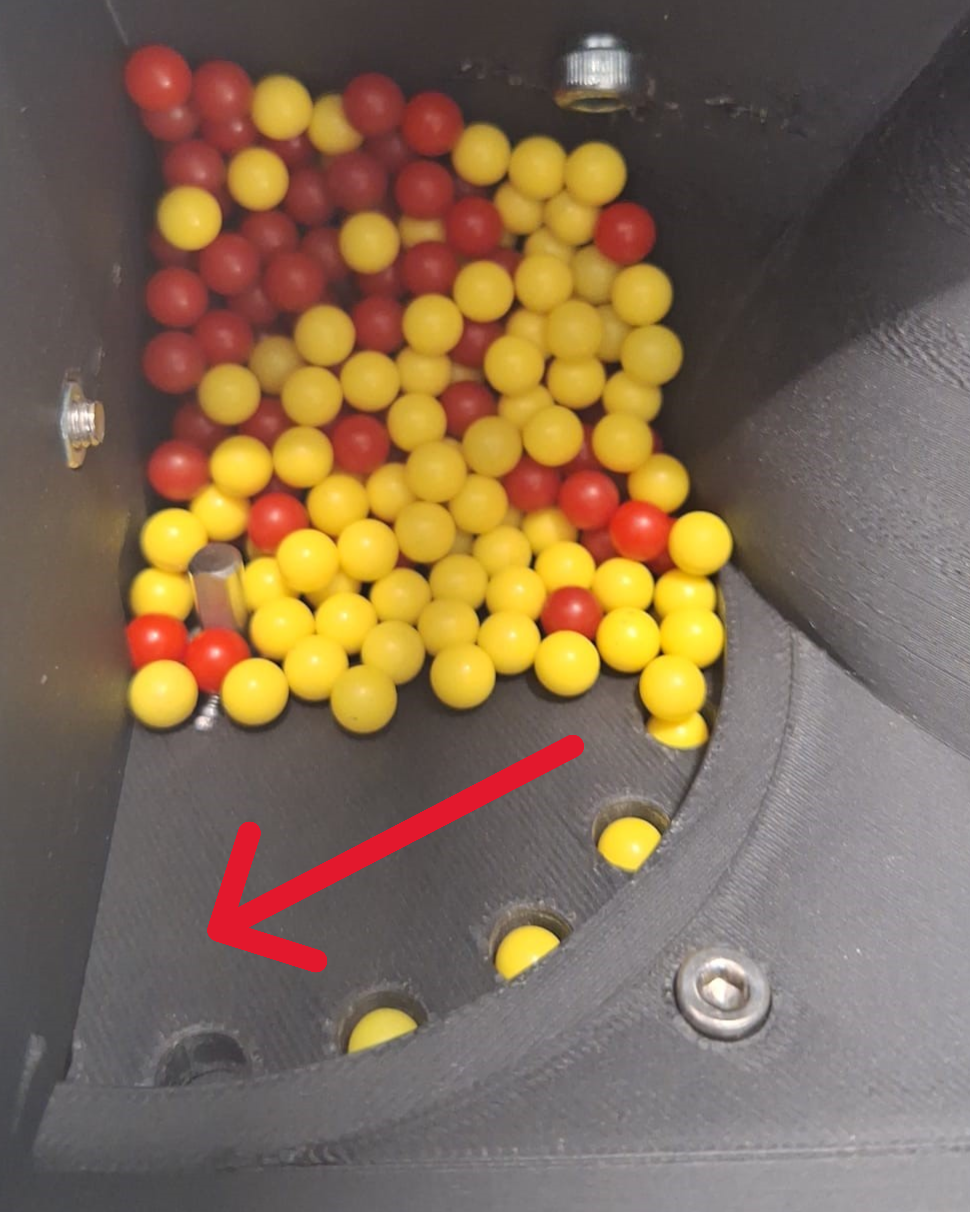
\includegraphics[width=0.8\textwidth]{figures/b15ba5c8-ba29-495a-9e40-18a8cdfba58f.PNG}
    \caption{Trichter mit Drehteller zur KugelrückführungTrichter mit Drehteller zur Kugelrückführung\cite{siemens2022}} 
    \label{fig:Trichter mit Drehteller zur Kugelrückführung} % Für spätere Verweise im Text.
    \vspace{0.5em} % Optional: Abstand zwischen Bildunterschrift und Zusatztext
    \small % Schriftgröße anpassen, falls gewünscht
\end{figure}

\section{Projekt SmartFactory-Anlage: Ergebnis}\label{sec:Projekt_SmartFactory-Anlage:_Ergebnis}

Der finale Funktionsumfang des Projekts lässt sich zum Zeitpunkt der Erstellung dieses Berichts noch nicht vollständig abschätzen, da einige 
Aspekte der Entwicklung und Implementierung noch in Arbeit sind. Dennoch konnte das Team bereits bedeutende Fortschritte erzielen und wesentliche 
Meilensteine gemäß den ursprünglichen Vorgaben und dem Projektplan erreichen. Besonders hervorzuheben ist, dass alle kritischen Fehler, die den 
Betrieb der Abfüllstation maßgeblich beeinträchtigen oder den Prozess unterbrechen konnten, erfolgreich identifiziert und behoben wurden. 
Lediglich kleinere Bugs, die keine direkte Auswirkung auf den kontinuierlichen Betrieb haben, verbleiben noch zur Bearbeitung. Damit wurde 
eines der zentralen Projektziele, die Robustheit der gesamten Anlage erheblich zu steigern, erfolgreich realisiert.

Der Fokus der weiteren Arbeiten liegt nun darauf, die Benutzerfreundlichkeit des Systems weiter zu verbessern und die Anlage so zu gestalten, 
dass sie zukünftig leicht erweitert und angepasst werden kann. Die Verbesserung der Bedienoberflächen, die Optimierung der Steuerungslogik und 
die Anpassung der Kommunikationsprozesse zwischen den Stationen sind dabei wichtige Arbeitsbereiche, die bereits angestoßen wurden.

Aus den regelmäßigen Teammeetings sowie dem wertvollen Feedback der Projektmitglieder und betreuenden Lehrkräfte geht klar hervor, dass auch an 
den anderen Stationen der Anlage signifikante Fortschritte erzielt wurden. Trotz der Herausforderungen, die sich durch die komplexen 
Abhängigkeiten der Systeme ergeben, konnte das Projektteam durch gezielte Koordination und klare Zielsetzungen einen stabilen Fortschritt 
sicherstellen. Sollte es dennoch vorkommen, dass der Projektfortschritt bis zum Abschluss des Praxissemesters nicht alle gesetzten Ziele 
vollständig erreicht, gewährleisten die sorgfältig erstellten Konzept- und Entwurfsdokumente eine solide Grundlage für die Weiterentwicklung 
des Projekts durch zukünftige Studierende. Diese Dokumente enthalten detaillierte Beschreibungen der bisherigen Arbeiten, der zugrunde liegenden 
Systemarchitektur sowie Empfehlungen für künftige Implementierungen.

Besonders bemerkenswert ist, dass durch die vorgenommenen Änderungen an der Abfüllstation nicht nur die Effizienz des Produktionsprozesses 
erheblich gesteigert werden konnte. Auch die Benutzerfreundlichkeit und Robustheit des gesamten Systems wurden signifikant verbessert. 
Die Reduktion von Störungen, die Erhöhung der Systemstabilität und die klar strukturierte Benutzerführung tragen dazu bei, dass die Anlage 
zuverlässiger und einfacher zu bedienen ist. Die ergriffenen Maßnahmen bilden somit eine wertvolle Grundlage für den langfristigen Erfolg 
des Projekts.
